\chapter{System topology}
%利用热力学原理进行定性分析。提炼出创新点。
\section{System topology design}
\subsection{Basic systems}

The objective of this research is to research the equipment of solar thermal power generation system, to propose, develop and optimize a solar thermal cascade system depending on the advantages and disadvantages of the solar thermal power generation systems. 
The research is based on the national cooperation project "Collaborative research on key technologies to produce electricity by cascade utilization solar thermal energy" as the background. 
There are three kinds of mature technologies been applied commercially -- parabolic trough, parabolic dish and solar tower. 
Considering the future deployment of solar cascade demo system, two solar thermal technologies, parabolic trough and parabolic dish, are chosen as the basic systems for the design of cascade solar thermal power system. For the cascade utilization of the high temperature of the parabolic receiver, air (or nitrogen) is used as the HTF to transfer the heat collected.
Figure~\ref{fig:PTPD} shows the schematic diagrams of a parabolic trough system and a parabolic dish system.

\begin{figure}[!ht]
\centering
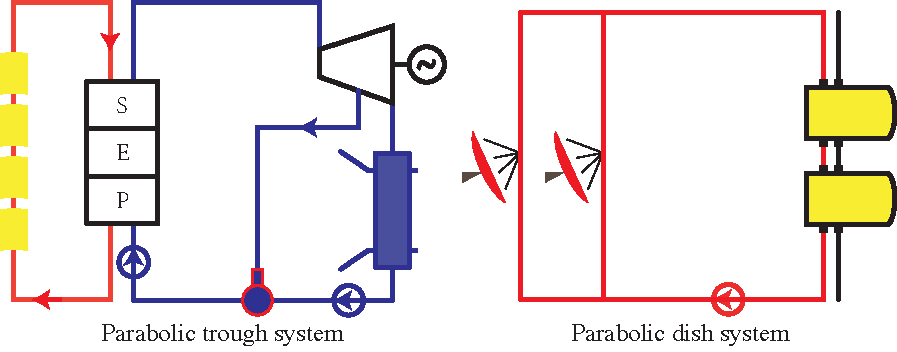
\includegraphics[width=0.8\textwidth]{fig/PTPD.pdf}
\caption{Schematic diagrams of a parabolic trough system and a parabolic dish system}\label{fig:PTPD}
\end{figure}

With different considerations (such as water Rankine cycle or ORC, combination of different systems, connection types of collectors, etc) of the cascade system topology, multiple combination topologies may be used for cascade systems. To get the most suitable system topology, these considerations will be analyzed in the following sections. 

\subsection{Rankine cycle fluid}

There are two important aspects to consider when selecting the working fluid of the Rankine cycle solar power system:
\begin{enumerate}
  \item Select the working fluid that is conducive to the optimization of the cycle efficiency
  
  For a Rankine cycle solar system, the collector efficiency reduces with operating temperature, and the Rankine cycle efficiency increases with operating temperature, there exists an optimal operating temperature as illustrated in Fig.~\ref{fig:Efficiency}. The working fluid should be conducive to achieve the optimal operating temperature.
  
  \begin{figure}[!ht]
\centering 
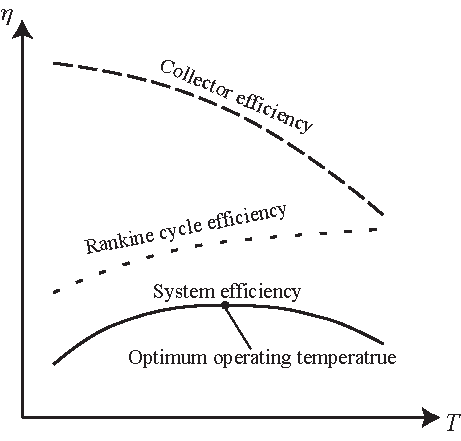
\includegraphics[width=0.7\textwidth]{fig/Efficiency}
\caption{Collector and Rankine cycle efficiency variation with operating temperature}\label{fig:Efficiency}
\end{figure}
  
  \item The working fluid state matches the heat transfer fluid state, if heat transfer fluid is used
  
  On the one hand, the operating temperature of the working fluid should be lower than the collecting temperature of the HTF. One the other hand, the operating temperature of the working fluid should not be much lower than the collecting temperature of the HTF, for this will cause large exerge loss during the heat exchange process.
  
\end{enumerate}

\begin{figure}[!ht]
\centering 
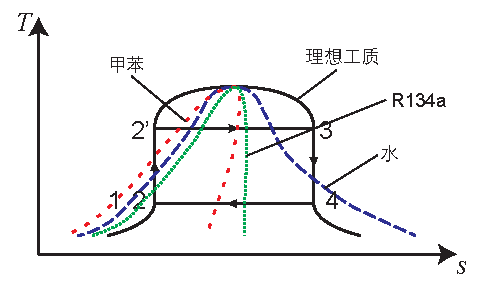
\includegraphics[width=0.7\textwidth]{fig/idealTs}
\caption{Collector and Rankine cycle efficiency variation with operating temperature}\label{fig:idealTs}
\end{figure}

An ideal working fluid would have the temperature entropy diagram given in Fig~\ref{fig:idealTs}. The following characteristics listed by Abbin and Leuenberger~\cite{Abbin1977} describe this fluid:
\begin{itemize}
  \item The heat capacity of the liquid phase should be small. This makes the curve 22' in Fig.~\ref{fig:idealTs} almost vertical.
  \item The critical point should be above the highest operating temperature to allow all heat to be added at that temperature.
  \item The vapor pressure at the highest operating temperature should be moderate for safety reasons and to reduce the cost of the equipment.
  \item The vapor pressure at the condensing temperature should be above atmospheric pressure to prevent air leakage into the system.
  \item The specific volume of the vapor at state 4 should be small to avoid large-diameter turbine wheels, casings, and heat exchangers.
  \item The saturated vapor curve 3-4 in fig.~\ref{fig:idealTs} should be vertical to avoid expansion into the wet vapor region (negative $ds/dT$) or expansion into the superheat region (positive $ds/dT$).
  \item For low-power turbine applications, the fluid should have a high molecular weight to minimize the rotational speed and/or the number of turbine stages and to allow for reasonable mass flow rates and turbine nozzle areas.
  \item The fluid should be liquid at atmospheric pressure and temperature for ease of handling and containment.
  \item The freezing point should be lower than the lowest ambient operating temperature.
  \item The fluid should have good heat-transfer properties, be inexpensive, thermally stable at the highest operating temperature, nonflammable, noncorrosive, nontoxic, and so on.
\end{itemize}

Water is the most commonly used fluid for Rankine cycle, it is mare mature to design Rankine cycle components for steam systems than any other liquid. It is inexpensive to use (although boiler-grade water must be highly distilled and thus costs more than tap water), sealing of the high-pressure portions of a Rankine cycle using steam is not critical. Non-flammability and ready availability of steam are additional advantages. Because it has a critical temperature and pressure of $374\,\mathrm{^\circ C} / 22.1\,\mathrm{MPa}$, it can be used for systems operating at fairly high temperatures with most of the heat addition (at constant temperature) and at moderate pressure. Figure~\ref{fig:TypicalSteamRankineSolarSystem} shows the schematic diagram of a typical steam Rankine cycle solar system.

\begin{figure}[!ht]
\centering 
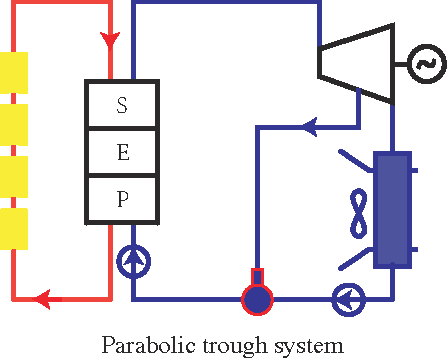
\includegraphics[width=0.7\textwidth]{fig/TypicalSteamRankineSolarSystem}
\caption{Schematic diagram of a typical steam Rankine cycle solar system}\label{fig:TypicalSteamRankineSolarSystem}
\end{figure}

There are some disadvantages for steam as the Rankine cycle fluid. The low temperature characteristics of steam are not ideal because the steam has a low vapor pressure (0.03$\,\mathrm{atm}$) and a very low density at ambient temperature. Therefore, sealing air from low pressure components is a major design problem.

The organic Rankine cycle can be used in the solar parabolic trough technology in place of the usual steam Rankine cycle. The ORC allows power generation at lower capacities and with a lower collector temperature, and hence the possibility for low-cost, small scale decentralized CSP units. Most organic fluids used in organic Rankine cycle are drying fluids. The vapor leaving the expander still contains heat that can be transferred to the compressed liquid stream because the turbine outlet temperature is above the condenser temperature. A vapor-to-liquid heat exchanger, known as a regenerator, is typically used for this purpose.
Fig.~\ref{fig:TypicalOrganicRankineSolarSystem} shows the schematic diagram of a typical organic Rankine cycle solar system. 

\begin{figure}[!ht]
\centering 
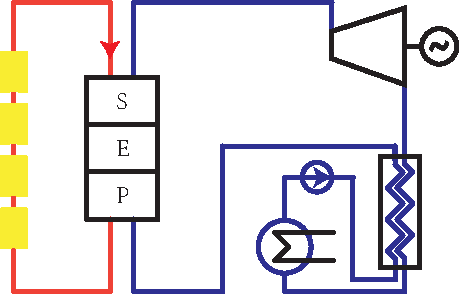
\includegraphics[width=0.7\textwidth]{fig/TypicalOrganicRankineSolarSystem}
\caption{Schematic diagram of a typical organic Rankine cycle solar system}\label{fig:TypicalOrganicRankineSolarSystem}
\end{figure}

Compared with steam for the Rankine cycle, it has the following advantages:
\begin{itemize}
  \item  Small turbine head allows for moderate shaft speed and a single- or two-stage design.
    \item Low volume ratio facilitates the flow path design.
    \item High volume flow and low velocity of sound results in reasonable flow areas.
    \item Low temperature drop during expansion reduces thermal stress problems.
    \item Dry expansion avoids blade erosion caused by vapor wetness.
    \item Low system pressure facilitates housing design.
  \end{itemize}

\subsection{Solar chimney}
Solar chimney, also known as solar updraft tower, directly (without concentration) uses the sun's heat to generate power. It uses solar radiation to increase the internal air temperature to form a flow to the chimney located at the middle of the roof. Fig.~\ref{fig:SolarChimney} shows the schematic of a typical solar chimney power plant. In this plant, air is heat by the green house effect under the translucent roof. As the roof is open at its periphery, air flows into the plant due to different density distribution. Hot air flows into the chimney because of buoyancy. An electricity-generating turbine is set in the path of the air current to convert the kinetic energy of the flowing air into electricity.

\begin{figure}[!ht]
\centering 
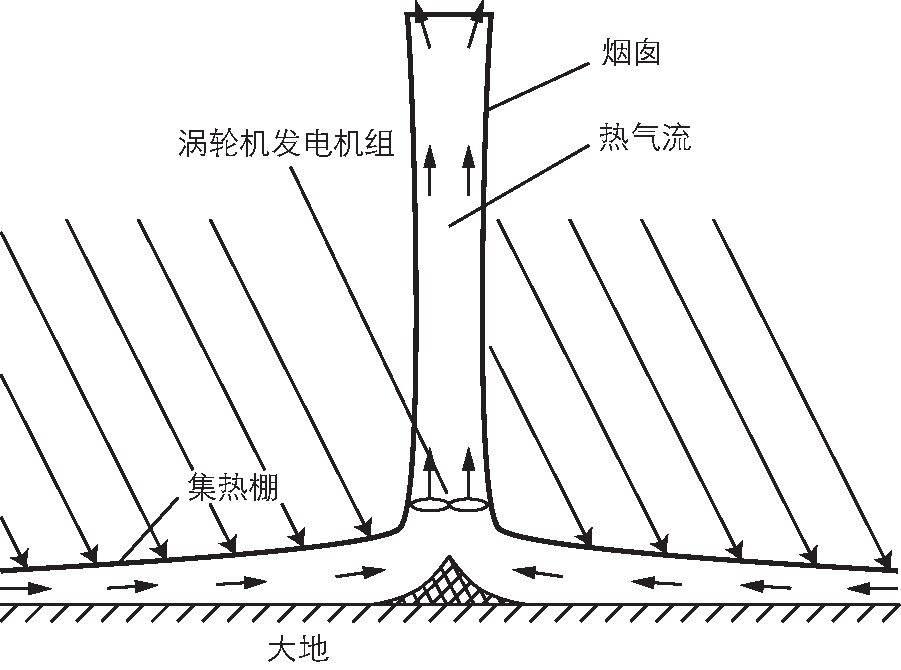
\includegraphics[width=0.7\textwidth]{fig/SolarChimney}
\caption{Schematic diagram of a solar chimney power plant}\label{fig:SolarChimney}
\end{figure}

The solar chimney can use the low temperature (low grade energy) for power generation. So the combination of parabolic trough system and solar chimney is considered an effective way for energy cascade utilization. In the combined system, the condenser in the Rankine cycle is air cooled. The fan blows the hot air that has cooled the condenser into the solar chimney power plant from its periphery. The hot air stream converges at the bottom of chimney, flows upward with the action of buoyancy and drives the turbine in the chimney.
Energy of the hot air can be utilized by the solar chimney. Fig.~\ref{fig:CombinedSolarChimney} shows an example of the combined system. 

\begin{figure}[!ht]
\centering 
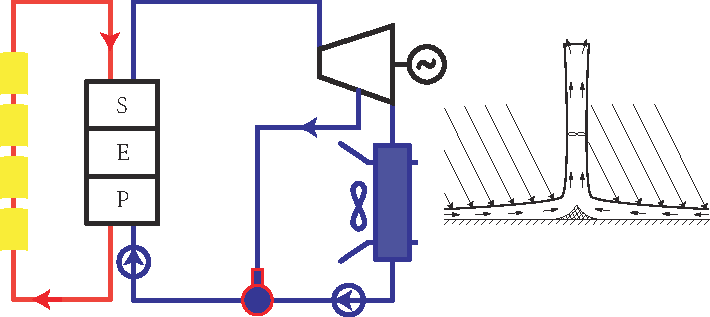
\includegraphics[width=0.7\textwidth]{fig/CombinedSolarChimney}
\caption{Schematic diagram of a combined solar trough and chimney power system}\label{fig:CombinedSolarChimney}
\end{figure}

However, the efficiency of solar chimney system is very low. Primary design data of solar chimney power plants with different location, different chimney height and collector height are shown in Table~\ref{tab:sc}~\cite{Bilgen2005}.

\begin{table}[htbp]
	\caption{Results of SEA models under specified parameters}
	\begin{center}
	\begin{tabular}{ccccc}
		\toprule
		&Ottawa    &Winnipeg    &Edmonton    &Schlaich\\
		\midrule
		Collector diameter (m)    &-&-&-&1110 \\
  Collector area ($\mathrm{m^2}$)    & 950000    & 950000&950000&950000\\
  Chimney height (m)    &123    &60    &    35&    547\\
  Collector height (m)    &848    &975    &1024    &    -\\
  Chimney diameter (m)    &54    &54    &54    &54\\
  Temperature rise in collector ($\mathrm{^\circ C}$)    &25.9    &25.9    &25.9    &25.9\\
  Updraught velocity (m/s)&9.1    &9.1    &9.1    &9.1\\
  Total pressure head (Pa)&518.3    &518.3    &518.3    &383.3\\
  Average efficiency\\
  Collector (\%)    &56.00    &56.00    &56.00    &56.24\\
  Chimney (\%)    &1.82    &1.82    &1.82    &1.45\\
  Turbine (\%)    &77.0    &77.0    &77.0    &77.0\\
  Whole system (\%)    &0.79    &0.79    &0.79    &0.63\\
		\bottomrule
	\end{tabular}
	\end{center}
	\label{tab:sc}
\end{table}

The preliminary design parameters in Table~\ref{tab:sc} are selected and determined for a nominal solar intensity of 1000$\,\mathrm{W/m^2}$ and the nominal plant power of 5$\,\mathrm{MW}$. From the table, it can be found that the chimney efficiency and total efficiency are very low and the technology is still in the development stage.

\subsection{Collector series connection}
Considering different heat collecting temperatures of different types of collectors, series connection of different types of collectors can be a feasible choice for solar cascade collection. Trough collectors and Fresnel collectors have better performance for lower temperature heat collection. Dish collectors and solar towers are more suitable for higher temperature heat collection. Serial connection utilize the advantages of different types of collectors. Figure~\ref{fig:SeriesCollector} shows an example of a cascade system using collector series connection. In this system, air, the HTF, is preheated by parabolic collectors before it flows into the parabolic dish collectors.

\begin{figure}[!ht]
\centering 
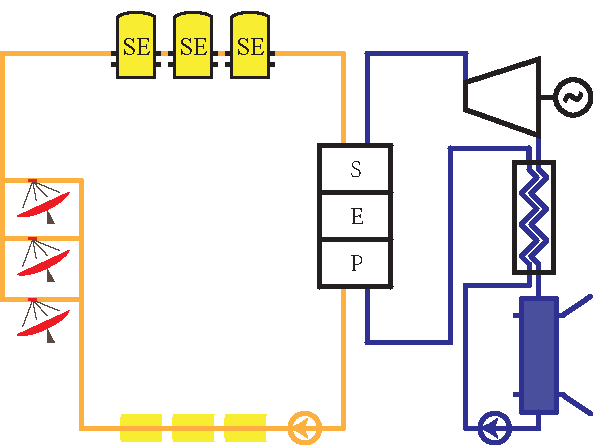
\includegraphics[width=0.7\textwidth]{fig/SeriesCollector}
\caption{Schematic diagram of a cascade system using collector series connection}\label{fig:SeriesCollector}
\end{figure}

\subsection{Direct steam generation}

All commercial parabolic trough solar plants implemented to date use heat-transfer fluid (typically synthetic oil or melton salt) in the solar field. It leads to high pressure drop, limits the oil (or salt) related equipment operation, maintenance and cost. Besides, the highest temperature of the Rankine cycle is limited by the oil (or salt) temperature. So generating steam in the receiver tubes (direct steam generation, DSG) of the solar collector is one of the directions to reduce the cost and increase the efficiency of the PTC systems. Fig.~\ref{fig:DSG} shows the schematic diagram of a typical DSG solar system.

\begin{figure}[!ht]
\centering 
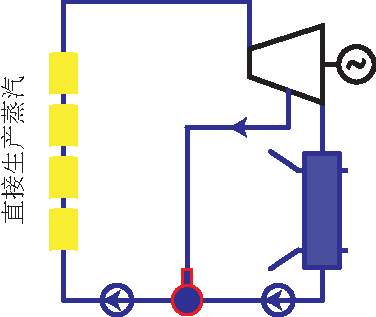
\includegraphics[width=0.7\textwidth]{fig/DSG}
\caption{schematic diagram of a typical solar system using receiver vapor generator}\label{fig:DSG}
\end{figure}

Generating vapor in the receiver of the solar collector has the advantage of having fewer components and no loss of temperature required with an intermediate transfer. With both liquid and vapor in a receiver, however, extreme care must be taken in the design of the receiver to ensure that the radiant flux incident on that portion of the receiver containing vapor is less than the flux incident in the regions with liquid and where boiling is taking place. This is because the heat-transfer coefficient into a liquid is significantly higher than into superheated vapor. For similar values of solar flux, burnout of the receiver walls could occur in the regions where vapor exists on the other side of the receiver wall.
Many concentrating collector designs require that the receiver change attitude while the collector tracks the sun. This change of attitude increases the chances of high flux on portions of the receiver containing vapor.
Two examples of solar Rankine power systems where the engine working fluid vapor is generated directly in the receiver are the Solar One Pilot Plant at Barstow, CA and the solar organic Rankine cycle module built by Ford Aerospace and Communications Corporation. Because Solar One is a central receiver system, the vertical-tube receiver remains stationary and liquid level control is relatively easy. The vertical tubes of the receiver are made of a material with a high melting point and thus can withstand high temperatures in the upper regions where vapor is being superheated. Tube burnout is avoided in the Ford Aerospace receiver design because the inner wall of the receiver is a copper shell with tubes wound around its exterior. The high thermal conductivity of the copper shell provides an averaging effect on receiver temperature, and superheat is attained without burnout of the receiver walls.

\subsection{Heat exchangers between different circuits}

Heat transfer between different circuits can be applied to cascade utilize the heat collected.

\subsection{Heat recovery between different cycles}

\section{System topology selection}

\subsection{Rankine cycle fluid}
\subsection{Solar chimney}
\subsection{Collector series connection}
\subsection{Direct steam generation}
\subsection{Heat exchangers between different circuits}